\documentclass[11pt]{article}

% Remove the "review" option to generate the final version.
% \usepackage{EMNLP2023}
\usepackage{EMNLP2023}

% Standard package includes
\usepackage{xeCJK}
\usepackage{setspace}
\usepackage{latexsym}

% For proper rendering and hyphenation of words containing Latin characters (including in bib files)
% \usepackage[T1]{fontenc}
% For Vietnamese characters
% \usepackage[T5]{fontenc}
% See https://www.latex-project.org/help/documentation/encguide.pdf for other character sets

% This is not strictly necessary, and may be commented out.
% However, it will improve the layout of the manuscript,
% and will typically save some space.
\usepackage{microtype}

% This is also not strictly necessary, and may be commented out.
% However, it will improve the aesthetics of text in
% the typewriter font.
\usepackage{inconsolata}

% \newcommand{\mh}{\textsc{mha}\xspace}
% \newcommand{\mq}{\textsc{mqa}\xspace}
% \newcommand{\gmq}{\textsc{gqa}\xspace}
\newcommand{\mh}{\textsc{MHA}\xspace}
\newcommand{\mq}{\textsc{MQA}\xspace}
\newcommand{\gmq}{\textsc{GQA}\xspace}
\newcommand{\fullgmq}{grouped-query\xspace}
\newcommand{\fullgmqcap}{Grouped-query\xspace}
\newcommand{\upprop}{\alpha}

\definecolor{niceblue}{rgb}{0, 0.46484375, 0.73046875} % Blue
\definecolor{gqcolor}{rgb}{0, 0.46484375, 0.73046875} % Blue
\definecolor{mhcolor}{rgb}{0.9296875, 0.3984375, 0.46484375} % red #EE6677
\definecolor{mqcolor}{rgb}{0.95, 0.52, 0.0} % tangerine #F28500
\definecolor{firstcolor}{rgb}{0.85, 0.75, 0.85} % Thistle #D8BFD8
\definecolor{randomcolor}{rgb}{1.0, 0.7, 0.28} % Pastel orange	#FFB347
\definecolor{meancolor}{rgb}{0.21, 0.46, 0.53} % Teal blue #367588
% meancolor

% #4477AA
\definecolor{darkgrey}{rgb}{0.33203125,0.33203125,0.33203125} % grey 

% Standard package includes
\usepackage{latexsym}
\usepackage{xspace}
\usepackage{amsmath}
\usepackage{tabularx}
\usepackage{multirow}
\usepackage{booktabs}


\usepackage{xcolor}
\definecolor{dgreen}{rgb}{0,0.5,0}

\usepackage{tikz}
\pgfdeclarelayer{background}
\pgfdeclarelayer{main}
\pgfsetlayers{background,main}
\usetikzlibrary{calc}
\usepackage{ifthen}

% Setup plots libraries
\usepackage{graphicx}
\usepackage{caption}
\usepackage{subcaption}
\usepackage{float}
\usepackage{stfloats}
\usepackage{tikz}
\usepackage{pgfplots}
\usepgfplotslibrary{fillbetween}
\usetikzlibrary{patterns}
\pgfplotsset{compat=1.8}

\newenvironment{customlegend}[1][]{%
    \begingroup
    % inits/clears the lists (which might be populated from previous
    % axes):
    \csname pgfplots@init@cleared@structures\endcsname
    \pgfplotsset{#1}%
}{%
    % draws the legend:
    \csname pgfplots@createlegend\endcsname
    \endgroup
}%

\def\addlegendimage{\csname pgfplots@addlegendimage\endcsname}

\setCJKmainfont[
  BoldFont=FZHei-B01,
  ItalicFont=FZKai-Z03,
  BoldItalicFont=FZFangSong-Z02,
  SmallCapsFont=FZShuSong-Z01
]{FZShuSong-Z01}
\setCJKsansfont[AutoFakeBold=1.2, AutoFakeSlant=0.15]{FZHei-B01}
\setCJKmonofont[AutoFakeBold=1.2, AutoFakeSlant=0.15]{FZHei-B01}
\setmainfont{Times New Roman}
\setmonofont[AutoFakeBold=1.2]{LMMono10}
\setstretch{1.2}
\captionsetup{font={small,it,stretch=1.2}}
\let\oldfootnotesize\footnotesize
\renewcommand{\footnotesize}{\oldfootnotesize\itshape}


% If the title and author information does not fit in the area allocated, uncomment the following
%
%\setlength\titlebox{<dim>}
%
% and set <dim> to something 5cm or larger.

\title{\gmq：从 Multi-Head 检查点训练广义 Multi-Query Transformer 模型}

\author{
Joshua Ainslie\thanks{\- \ 同等贡献。},~ James Lee-Thorp\footnotemark[1],~ Michiel de Jong\footnotemark[1] \ \footnotemark[2]\thanks{\- \ University of Southern California。工作完成于 Google Research。} \\
{\bf Yury Zemlyanskiy},~ {\bf Federico Lebr\'{o}n},~ {\bf Sumit Sanghai}
  \AND
  {\rm \Large Google Research}\\
  }
% \author{Placeholder}

\begin{document}
\maketitle
\begin{abstract}
Multi-query 注意力 (\mq) 仅使用单个 key-value 头，可显著加速解码器推理。然而，\mq 可能导致质量下降，而且仅为更快推理而单独训练一个模型也未必理想。我们 (1) 提出一种方案，使用原始预训练计算量的 5\%，将已有的 multi-head 语言模型检查点继续训练为采用 \mq 的模型，并且 (2) 引入 \fullgmq 注意力 (\gmq)，它是 multi-query 注意力的一种泛化形式，使用中间数量的 key-value 头，即多于一个但少于 query 头数量。我们表明，经过继续训练的 \gmq 能以接近 \mq 的速度达到接近 multi-head 注意力的质量。

\end{abstract}

\section{引言}
\label{section:intro}

对于 Transformer 模型而言，自回归解码器推理是一个严重瓶颈，因为在每个解码步骤都需要加载解码器权重以及所有注意力的 key 和 value，从而产生内存带宽开销~\citep{shazeer2019mq, palminference, dejong2022fido}。通过 \emph{multi-query 注意力}~\citep{shazeer2019mq}，可以大幅降低加载 key 和 value 所需的内存带宽；该方法使用多个 query 头，但只使用单个 key 头和 value 头。

然而，multi-query 注意力 (\mq) 可能导致质量下降和训练不稳定，而且分别训练针对质量和推理优化的模型未必可行。此外，尽管一些语言模型已经使用 multi-query 注意力，例如 PaLM~\citep{palm}，但许多模型并未采用，包括 T5~\citep{t5} 和 LLaMA~\citep{llama} 等公开可用的语言模型。

本文围绕大语言模型的更快推理提出两项贡献。首先，我们表明，带有 multi-head 注意力 (\mh) 的语言模型检查点可以用原始训练计算量的一小部分进行 \emph{继续训练}~\citep{sparsemoe}，从而使用 \mq。这提供了一种高性价比的方法，可从高质量的 \mh 检查点获得快速的 multi-query 模型。

其次，我们提出 \fullgmq 注意力 (\gmq)，它介于 multi-head 和 multi-query 注意力之间，在 \emph{每个 query 头子组}中共享单个 key 头和 value 头。我们表明，经过继续训练的 \gmq 在几乎达到 multi-query 注意力速度的同时，获得接近 multi-head 注意力的质量。

\section{方法}
\label{section:method}



\subsection{继续训练}

从 multi-head 模型生成 multi-query 模型分为两步：首先转换检查点，其次进行额外预训练，使模型适应新的结构。图 \ref{fig:recycling} 展示了将 multi-head 检查点转换为 multi-query 检查点的过程。我们将 key 头和 value 头的投影矩阵平均池化为单个投影矩阵，并发现这比选择单个 key 头和 value 头，或从头随机初始化新的 key 头和 value 头效果更好。

\begin{figure}[ht]
    \centering
    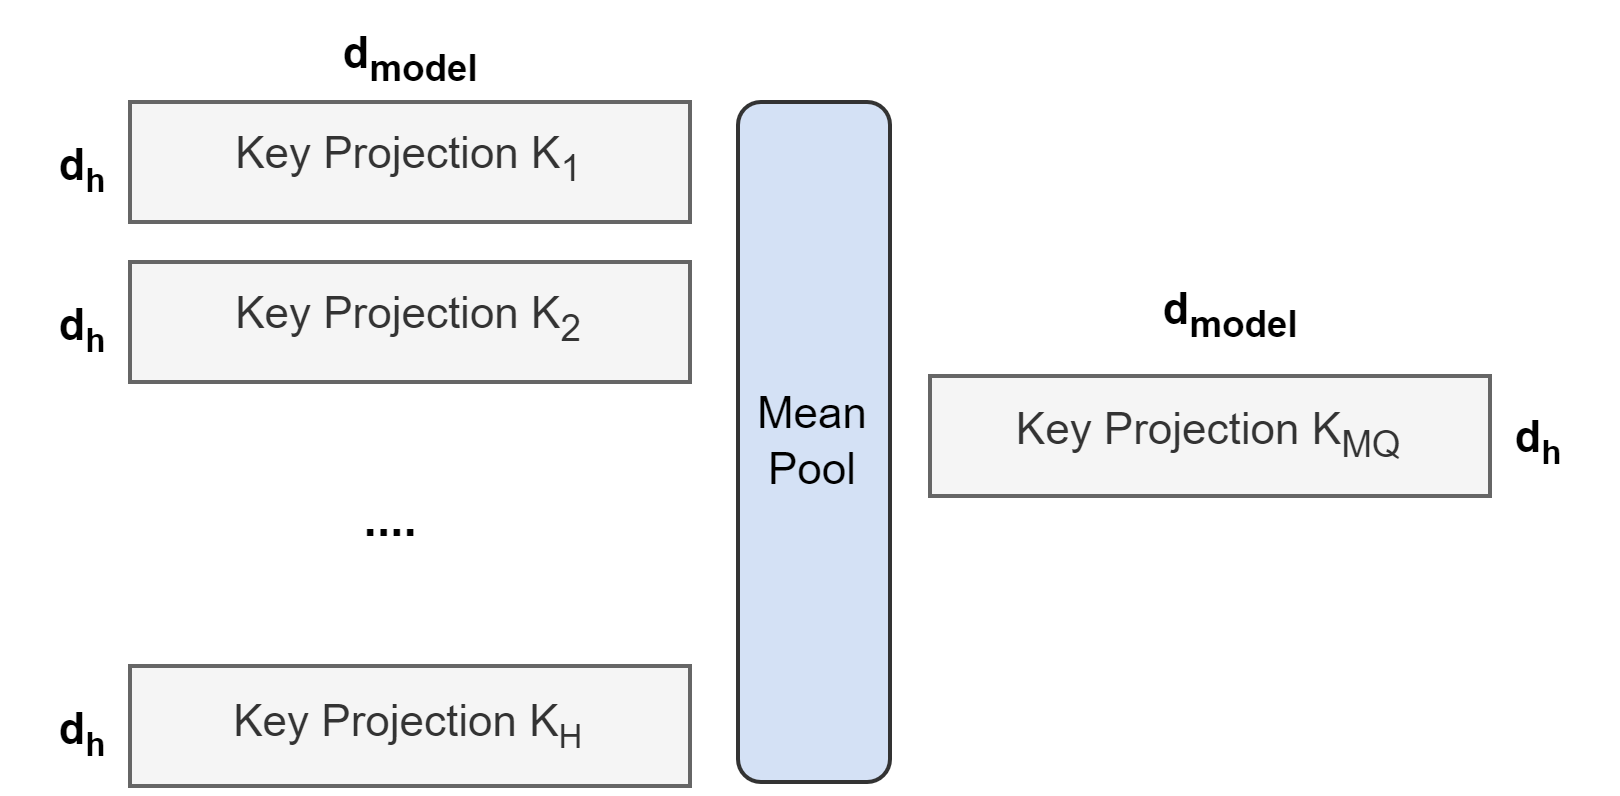
\includegraphics[width=0.95\columnwidth]{images/recycling.png}
    \caption{从 multi-head 注意力转换为 multi-query 注意力的概览。来自所有头的 key 和 value 投影矩阵被平均池化为单个头。}
    \label{fig:recycling}
\end{figure}


随后，转换后的检查点使用相同的预训练方案，再训练原始训练步数的一小部分 $\upprop$。

\subsection{\fullgmqcap 注意力}
\begin{figure*}[t]
    \centering
    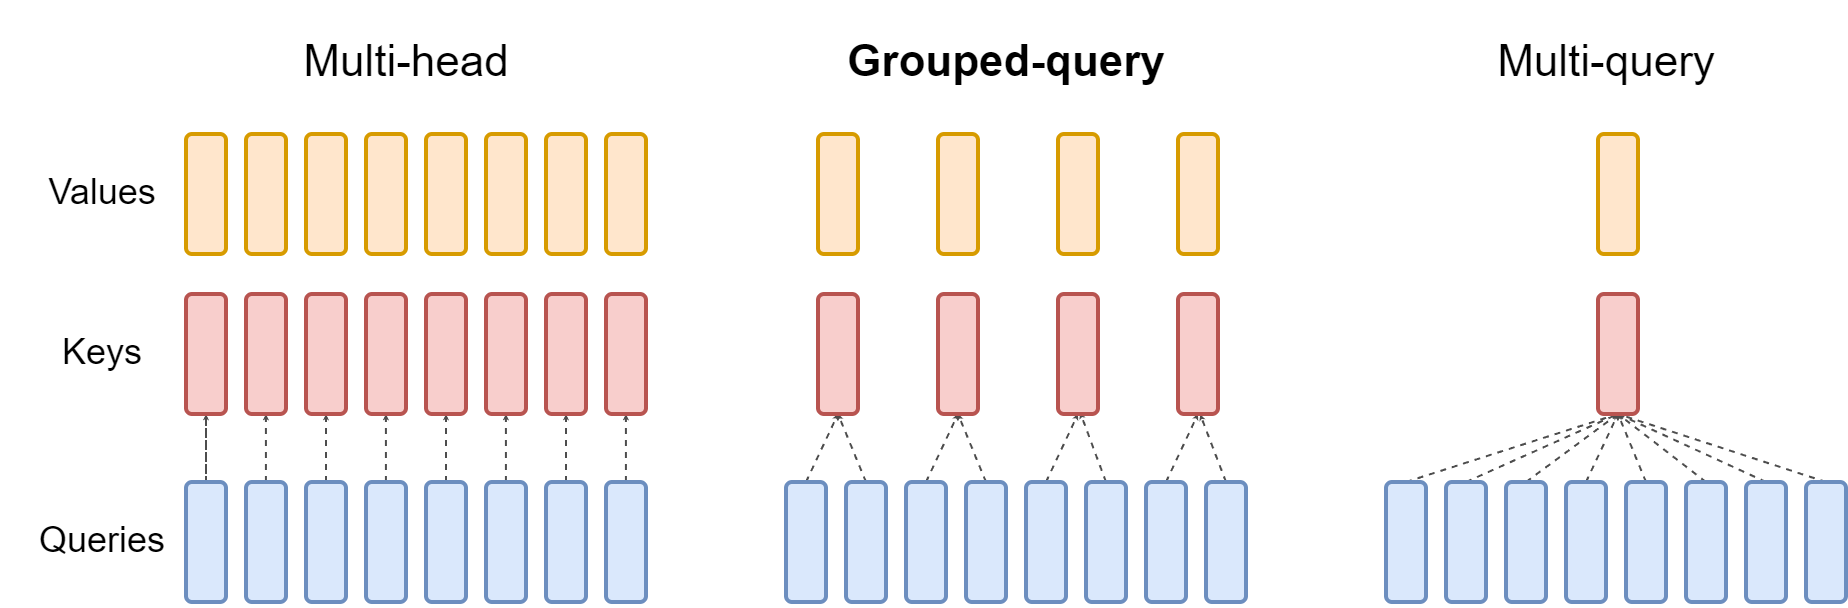
\includegraphics[width=0.9\textwidth]{images/gmq_architecture.png}
    \caption{\fullgmq 方法概览。Multi-head 注意力包含 H 个 query 头、key 头和 value 头。Multi-query 注意力在所有 query 头之间共享单个 key 头和 value 头。Grouped-query 注意力则为每个 query 头的 \emph{group} 共享单个 key 头和 value 头，从而在 multi-head 和 multi-query 注意力之间进行插值。}
    \label{fig:gmq_architecture}
\end{figure*}

\fullgmqcap 注意力将 query 头划分为 $G$ 个 \emph{组}，每组共享一个 key 头和一个 value 头。 \gmq-\textsc{g} 表示具有 $G$ 个组的 \fullgmq。 \gmq-$1$ 只有一个组，因此只有一个 key 头和 value 头，等价于 \mq；而 \gmq-\textsc{h} 的组数等于头数，等价于 \mh。图 \ref{fig:gmq_architecture} 展示了 \fullgmq 注意力与 multi-head/multi-query 注意力的比较。将 multi-head 检查点转换为 \gmq 检查点时，我们通过对该组内所有原始头进行平均池化，构造每个组的 key 头和 value 头。

中间数量的组会得到一个插值模型，其质量高于 \mq，速度快于 \mh，并且如我们将展示的那样，形成了有利的权衡。从 \mh 转为 \mq 会将 $H$ 个 key 头和 value 头减少为单个 key 头和 value 头，使 key-value 缓存大小以及需要加载的数据量减少 $H$ 倍。然而，更大的模型通常会增加头数，因此 multi-query 注意力会在内存带宽和容量上带来更激进的削减。 \gmq 使我们能在模型规模增大时，保持带宽和容量按相同比例下降。

此外，较大模型受注意力内存带宽开销的相对影响更小，因为 KV-cache 随模型维度线性增长，而模型 FLOPs 和参数随模型维度的平方增长。最后，大模型的标准分片会按照模型分区数量复制单个 key 头和 value 头~\citep{palminference}；\gmq 消除了这种分区方式带来的浪费。因此，我们预期 \gmq 对较大模型会呈现特别好的权衡。

需要指出的是，\gmq 并未应用于编码器 self-attention 层；编码器表征是并行计算的，因此内存带宽通常不是主要瓶颈。

\section{实验}
\label{section:experiments}

\subsection{实验设置}

\paragraph{配置}
所有模型均基于 T5.1.1 架构~\citep{t5}，并使用 JAX~\citep{jax}、Flax~\citep{flax} 和 Flaxformer\footnote{\url{https://github.com/google/flaxformer}} 实现。在主要实验中，我们考虑带有 multi-head 注意力的 T5 Large 和 XXL，以及经过继续训练、带有 multi-query 和 grouped-query 注意力的 T5 XXL 版本。我们使用 Adafactor 优化器，并采用与 T5~\citep{t5} 相同的超参数和学习率调度。我们将 \mq 和 \gmq 应用于解码器 self-attention 和 cross-attention，但不应用于编码器 self-attention。

\paragraph{继续训练}

继续训练模型从公开的 T5.1.1 检查点初始化。key 头和 value 头被平均池化为相应的 \mq 或 \gmq 结构，随后使用来自~\citep{t5} 的原始预训练设置和数据集，再训练原始预训练步数的 $\upprop$ 比例。当 $\upprop=0.05$ 时，训练大约需要 600 个 TPUv3 芯片日。

\paragraph{数据}
我们在摘要数据集 CNN/Daily Mail~\citep{cnn}、arXiv 和 PubMed~\citep{arxiv}、MediaSum~\citep{mediasum} 以及 Multi-News~\citep{multinews}，翻译数据集 WMT 2014 English-to-German，以及问答数据集 TriviaQA~\citep{triviaqa} 上进行评估。我们没有在 GLUE~\citep{glue} 等常用分类基准上评估，因为自回归推理不太适用于这些任务。

\paragraph{微调}

对于微调，所有任务均使用 0.001 的恒定学习率、128 的批大小和 0.1 的 dropout 率。CNN/Daily Mail 和 WMT 使用输入长度 512、输出长度 256。其他摘要数据集使用输入长度 2048、输出长度 512。最后，TriviaQA 使用输入长度 2048、输出长度 32。我们训练至收敛，并选择开发集性能最高的检查点。推理时使用贪心解码。

\paragraph{计时}
我们报告每个 TPUv4 芯片上每个样本的时间，该时间由 xprof~\citep{xprof} 测得。在计时实验中，我们使用 8 个 TPU，并采用每个 TPU 最多可容纳 32 个样本的最大批大小，同时为每个模型分别优化并行化设置。
\begin{table*}[ht!]
\centering
\footnotesize
\begin{tabular}{l|cc|ccccccccc}
\toprule
\textbf{Model} &  \textbf{T\textsubscript{infer}}& \textbf{Average} & \textbf{CNN}  &  \textbf{arXiv} & \textbf{PubMed}  &\textbf{MediaSum} & \textbf{MultiNews} &  \textbf{WMT} &  \textbf{TriviaQA}  \\
\midrule
  & \textbf{s} &  & \textbf{R\textsubscript{1}}  & \textbf{R\textsubscript{1}} &  \textbf{R\textsubscript{1}} & \textbf{R\textsubscript{1}}  &\textbf{R\textsubscript{1}} & \textbf{BLEU} & \textbf{F1}   \\
 \midrule
  \mh-Large &  0.37 & 46.0 & 42.9 & 44.6 & 46.2 & 35.5 & 46.6 & 27.7 & 78.2 \\
 \mh-XXL & 1.51 & 47.2 &  43.8 & 45.6 & 47.5 & 36.4 & 46.9 & 28.4 & 81.9 \\
 \mq-XXL  & 0.24 & 46.6 & 43.0 & 45.0 & 46.9 & 36.1 & 46.5 & 28.5 & 81.3 \\
 \gmq-8-XXL & 0.28  & 47.1 & 43.5 & 45.4 & 47.7 & 36.3 & 47.2 & 28.4 & 81.6 \\
\midrule
\bottomrule
\end{tabular}
\caption{Inference time and average dev set performance comparison of T5 Large and XXL models with multi-head attention, and 5\% uptrained T5-XXL models with multi-query and grouped-query attention on summarization datasets CNN/Daily Mail, arXiv, PubMed, MediaSum, and MultiNews, translation dataset WMT, and question-answering dataset TriviaQA.}
\label{table:headline_results}
\end{table*}
\begin{figure}[ht]
\centering
\hspace{-0.5cm}
\begin{tikzpicture}
\begin{axis}[
width=0.98\columnwidth,
xmin=0.0, xmax=1.95,
ymin=45.65, ymax=47.40,
ylabel={Performance},
xlabel={Time per sample (ms)},
legend columns=1,
legend cell align=left,
legend style={
    anchor=south,
    at={(0.84, 0.05)},
},
]
\addplot[only marks, mark=*, mark options={draw=mhcolor, fill=mhcolor, scale=2}] coordinates {
    (0.372, 45.95)
    (1.514, 47.206)
};
\node at (axis cs:0.372,45.95) [anchor= north west, color=darkgrey] {\small{MHA-Large}};            
\node at (axis cs:1.514,47.206) [anchor= north east, color=darkgrey] {\small{MHA-XXL}};            
\addplot[only marks, mark=*, mark options={draw=mqcolor, fill=mqcolor, scale=2}] coordinates {
    (0.239, 46.571)
};
\node at (axis cs:0.239,46.548) [anchor= north west, color=darkgrey] {\small{MQA-XXL}};            
\addplot[only marks, mark=*, mark options={draw=gqcolor, fill=gqcolor, scale=2}] coordinates {
    (0.275, 47.136)
};
\node at (axis cs:0.275,47.136) [anchor= north west, color=darkgrey] {\small{GQA-XXL}};            
\end{axis}
\end{tikzpicture}
    \caption{{\bf 与 \mh 相比，经过继续训练的 \mq 实现了有利的权衡，其质量高于且速度快于 \mh-Large，而 \gmq 在获得相近速度提升的同时实现了更好的性能，质量与 \mh-XXL 相当。} 对采用 multi-head 注意力的 T5-Large 和 T5-XXL，以及经过 5\% 继续训练、采用 \mq 和 \gmq-8 注意力的 T5-XXL，展示所有任务平均性能随每个样本平均推理时间的变化。}
    \label{fig:perf_vs_time}
\end{figure}

\subsection{主要结果}

图 \ref{fig:perf_vs_time} 展示了 \mh T5-Large 和 T5-XXL，以及继续训练比例 $\upprop = 0.05$ 的 \mq 和 \gmq-$8$ XXL 模型，在所有数据集上平均性能随平均推理时间变化的关系。我们可以看到，相比 \mh 模型，更大的继续训练 \mq 模型提供了有利的权衡，其质量高于 \mh-Large，推理也更快。此外，\gmq 带来了显著的额外质量收益，在接近 \mq 速度的同时达到接近 \mh-XXL 的性能。表 \ref{table:headline_results} 给出了所有数据集的完整结果。




\subsection{消融实验}

本节通过实验研究不同建模选择的影响。我们在具有代表性的任务子集上评估性能：CNN/Daily Mail，即 short-form summarization；MultiNews，即 long-form summarization；以及 TriviaQA，即 question-answering。
\begin{figure}[ht]
\centering
\hspace{-0.5cm}
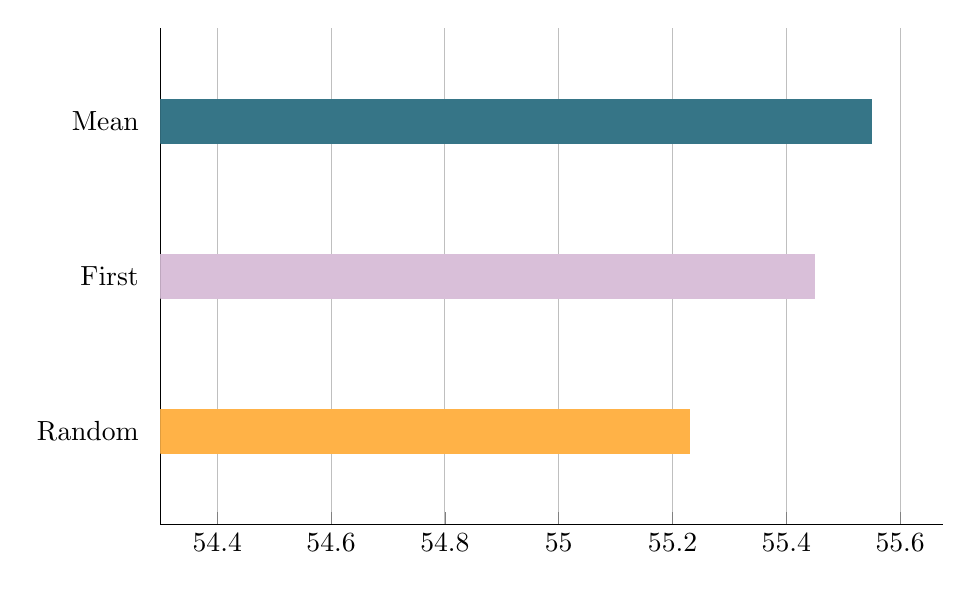
\begin{tikzpicture}
\begin{axis}[
    xbar,
    bar shift=0pt,
    enlarge y limits=0.3,
    width=0.95\columnwidth,
    height=0.65\columnwidth,
    bar width=16pt,
    major y tick style = transparent,    
    xmajorgrids = true,
    symbolic y coords={Mean, First, Random},
    yticklabels={Mean, First, Random},   
    ytick={Mean, First, Random},
    y dir=reverse,
    xmin=54.3,
    axis y line*=none,
    axis x line*=bottom,
]
    \addplot[style={meancolor,fill=meancolor,mark=none}]
        coordinates {(55.55,Mean)};
    \addplot[style={firstcolor,fill=firstcolor,mark=none}]
        coordinates {(55.45,First)};             
    \addplot[style={randomcolor,fill=randomcolor,mark=none}]
        coordinates {(55.23,Random)};
  
\end{axis}
\end{tikzpicture}        
    \caption{T5-Large 以比例 $\alpha=0.05$ 继续训练为 \mq 时，不同检查点转换方法的性能比较。`Mean' 对 key 头和 value 头进行平均池化，`First' 选择第一个头，`Random' 从头初始化头。}
    \label{fig:conversion_methods}
\end{figure}


\paragraph{检查点转换}
图 \ref{fig:conversion_methods} 比较了不同检查点转换方法的性能。平均池化的效果似乎最好，其次是选择单个头，然后是随机初始化。直观来看，结果排序与从预训练模型中保留信息的程度一致。



\paragraph{继续训练步数}
图 \ref{fig:uptraining_steps} 展示了带有 \mq 和 \gmq 的 T5 XXL 性能如何随继续训练比例变化。首先，我们注意到 \gmq 在转换后已经达到合理性能，而 \mq 需要继续训练才具备实用性。 \mq 和 \gmq 都能从 5\% 的继续训练中获益，但从 10\% 开始收益递减。

\begin{figure}[ht]
\centering
        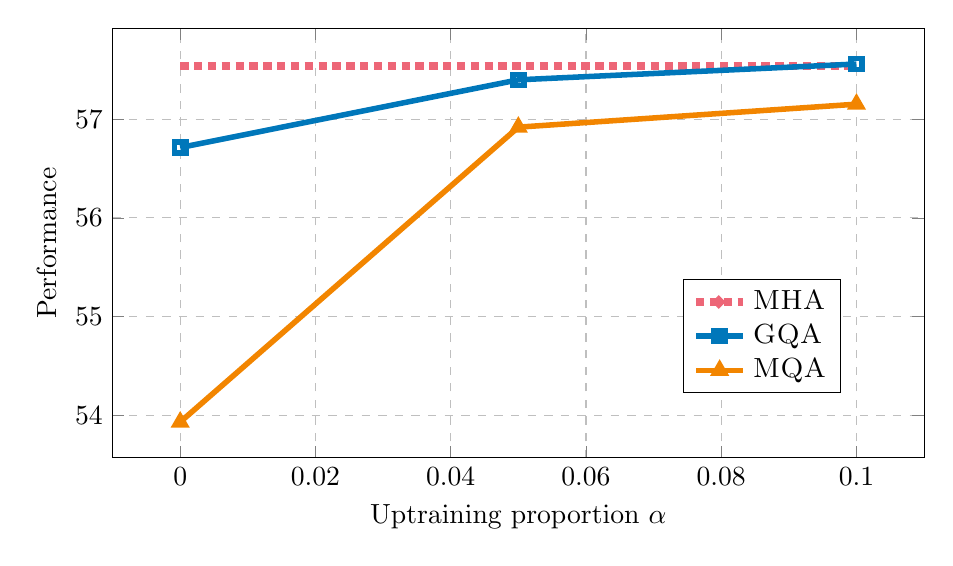
\begin{tikzpicture}[scale=1.0]
            \begin{axis}[
            scale only axis,
            width=0.85\columnwidth,
            height=0.45\columnwidth,
            ylabel={Performance},
            xlabel={Uptraining proportion $\upprop$},
            mark=x,
            xticklabel style={
                /pgf/number format/fixed,
                /pgf/number format/precision=2
            },            
            ymajorgrids=true,
            xmajorgrids=true,
            xminorticks=true,
            grid style=dashed,
            legend columns=1,
            legend cell align=left,
            legend style={
                anchor=south,
                at={(0.8, 0.15)},
            },
        ]
            \addplot[color=mhcolor,mark size=2pt,line width=3, dotted] table {
                0 57.537
            	0.1 57.537
            };        
            \addplot[color=gqcolor,mark=square,mark size=2pt,line width=2] table {
                0 56.713
                0.05 57.4
            	0.1 57.56
            };            
            \addplot[color=mqcolor,mark=triangle,mark size=2pt,line width=2] table {

                0 53.93
                0.05 56.92
            	0.1 57.153            	
            };
            \legend{\mh, \gmq, \mq}
            \end{axis}
        \end{tikzpicture}
    \caption{采用 \mq 和 \gmq-8 的 T5 XXL 模型性能随 uptraining 比例的变化。}
    \label{fig:uptraining_steps}
\end{figure}

\paragraph{组数}

图 \ref{fig:time_groups} 展示了 \gmq 组数对推理速度的影响。对于较大模型，KV cache 带来的内存带宽开销约束较弱~\citep{shazeer2019mq}，而由于头数增加，key-value 大小的减少更加显著。因此，从 \mq 开始增加组数最初只会带来轻微减速，但随着接近 \mh，成本会逐渐上升。我们选择 8 个组作为较优的折中点。


\begin{figure}[ht]
\centering
        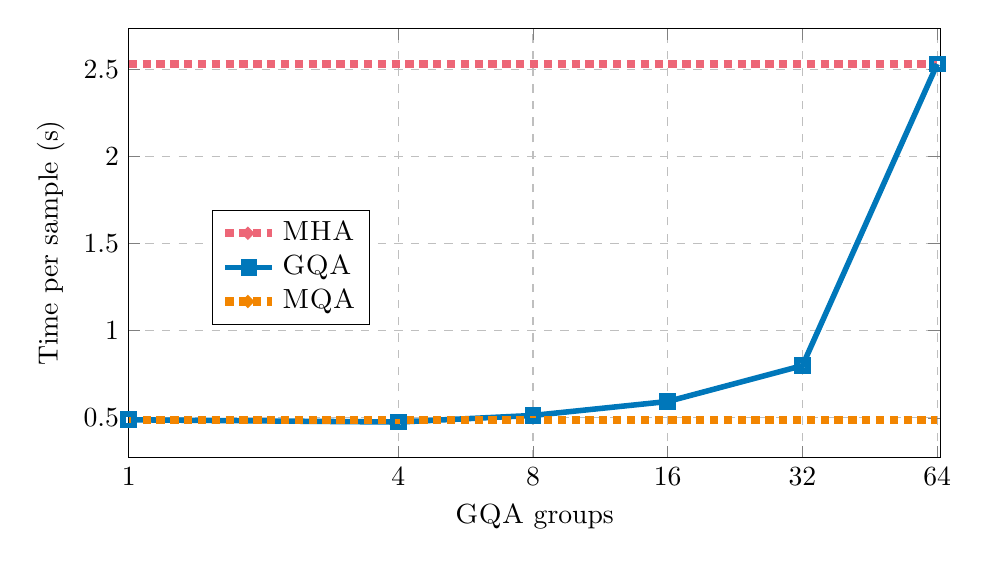
\begin{tikzpicture}[scale=1.0]
            \begin{axis}[
            scale only axis,
            xmode=log,
            width=0.85\columnwidth,
            height=0.45\columnwidth,
            ylabel={Time per sample (s)},
            xlabel={\gmq groups},
            mark=x,
            xmin=1,
            xmax=65,
            xtick={1, 4, 8, 16, 32, 64},
            xticklabels={1, 4, 8, 16, 32, 64},
            clip=false,
            ymajorgrids=true,
            xmajorgrids=true,
            xminorticks=true,
            grid style=dashed,
            legend columns=1,
            legend cell align=left,
            legend style={
                anchor=south,
                at={(0.2, 0.31)},
            },
        ]
            \addplot[color=mhcolor,mark size=2pt,line width=3, dotted] table {
                1 2.531
            	64 2.531
            };        
            \addplot[color=gqcolor,mark=square,mark size=2pt,line width=2] table {
                1 0.489
                4 0.476
                8 0.514
                16 0.594
                32 0.800
                64 2.531            

            };            
            \addplot[color=mqcolor,mark size=2pt,line width=3, dotted] table {
                1 0.489
            	64 0.489
            };
            \legend{\mh, \gmq, \mq}
            \end{axis}
        \end{tikzpicture}
    \caption{在输入长度为 2048、输出长度为 512 时，\gmq-XXL 每个样本的时间随 \gmq 组数的变化。从 1 组（\mq）增加到 8 组只带来适度的推理开销，但继续增加组数的成本会逐步上升。}
    \label{fig:time_groups}
\end{figure}


\section{相关工作}

本文聚焦于通过降低加载 key 和 value 产生的内存带宽开销~\citep{roofline}，在解码器质量和推理时间之间取得更好的权衡。 \citet{shazeer2019mq} 最早提出通过 multi-query 注意力降低这种开销。后续工作表明，multi-query 注意力对长输入尤其有帮助~\citep{palminference, dejong2022fido}。 \citet{gqamrabe} 独立开发了 GQA 并提供了公开实现。其他工作也探索了为计算效率而对注意力头分组~\citep{grouptrans, gmha, pillars}，但没有特别关注决定内存带宽开销的 key-value 头。

已有许多其他方法被提出，用于降低来自 key、value 以及参数的内存带宽开销。Flash 注意力~\citep{flashattention} 通过组织注意力计算来避免物化二次规模的注意力分数，从而减少内存并加速训练。量化~\citep{int8, gptq} 通过降低精度来减小权重和激活的大小，其中也包括 key 和 value。模型蒸馏~\citep{distill, distillsurvey} 则在给定精度下降低模型大小，使用由较大模型生成的数据来微调较小模型。Layer-sparse cross-attention \citep{dejong2022fido} 移除了大多数 cross-attention 层，而这些层构成长输入的主要开销。Speculative sampling~\citep{specchen, specleviathan} 使用较小模型提出多个 token，再由较大模型并行打分，从而缓解内存带宽瓶颈。

最后，我们提出的继续训练过程受到 \citet{sparsemoe} 的启发，该工作将标准 T5 检查点继续训练为稀疏激活的 Mixture-of-Experts 模型。

\label{section:related}

\section{结论}
\label{section:conclusion}

语言模型的推理成本高，主要是因为加载 key 和 value 会带来内存带宽开销。Multi-query 注意力以降低模型容量和质量为代价减少了这种开销。我们提出使用原始预训练计算量的一小部分，将 multi-head 注意力模型转换为 multi-query 模型。此外，我们引入 grouped-query 注意力，它介于 multi-query 和 multi-head 注意力之间，能够以接近 multi-query 注意力的速度达到接近 multi-head 的质量。

\section*{局限性}

本文聚焦于缓解加载 key 和 value 产生的内存带宽开销。当生成较长序列时，这种开销最为重要，而此类序列的质量本身也难以评估。对于摘要任务，我们使用 Rouge 分数，但我们知道这是一种有缺陷的评估，无法呈现完整情况；因此，很难确定我们的权衡一定正确。由于计算资源有限，我们也没有将 XXL \gmq 模型与从头训练的可比模型进行比较，因此无法得知继续训练相对于从头训练的相对性能。最后，我们仅在 encoder-decoder 模型上评估了继续训练和 \gmq 的影响。近来，decoder-only 模型极为流行，并且由于这些模型没有分离的 self-attention 和 cross-attention，我们预期 \gmq 相比 \mq 会有更强优势。


\section*{致谢}
我们感谢 Santiago Onta\~{n}\'{o}n、Afroz Mohiuddin、William Cohen 以及 Google Research 的其他同事提供富有洞见的建议与讨论。

\bibliography{custom}
\bibliographystyle{acl_natbib}


\clearpage
\appendix

\section{训练稳定性}

我们发现，multi-query 注意力可能在微调期间导致训练不稳定，尤其是在与长输入任务结合时。我们从头训练了多个带有 multi-query 注意力的 T5-Large 模型。每种情况下，预训练都会出现频繁的损失尖峰，并且最终模型在长输入任务上微调时会立即发散。经过继续训练的 multi-query 注意力模型更稳定，但仍表现出较高方差，因此对于不稳定任务上的 multi-query 模型，我们报告三次微调运行的平均性能。然而，经过继续训练的 grouped-query 注意力模型似乎是稳定的，因此我们没有进一步研究 multi-query 不稳定性的根本原因。

\end{document}
